%%%%%%%%%%%%%%%%%%%%%%%%%%%%%%%%%%%%%%%%%%%%%%%%%%%%%%%%%%%%%%%%%%%%%
%
% CSCI 1430 Written Question Template
%
% This is a LaTeX document. LaTeX is a markup language for producing documents. 
% You will fill out this document, compile it into a PDF document, then upload the PDF to Gradescope. 
%
% To compile it into a PDF you can:
% - Use vscode! Install a LaTeX distribution (all common OS): http://www.latex-project.org/get/ 
% + VSCode extension: https://marketplace.visualstudio.com/items?itemName=James-Yu.latex-workshop
% - Use an online tool: https://www.overleaf.com/ - most LaTeX packages are pre-installed here (e.g., \usepackage{}).
%
% If you need help with LaTeX, please come to office hours.
% Or, there is plenty of help online:
% https://en.wikibooks.org/wiki/LaTeX
%
% Good luck!
% The CSCI1430 staff
%
%%%%%%%%%%%%%%%%%%%%%%%%%%%%%%%%%%%%%%%%%%%%%%%%%%%%%%%%%%%%%%%%%%%%%

\documentclass{csci1430}

\begin{document}
\title{Homework 3 Written Questions}
\HomeworkShortName{HW3}
\maketitle

\writeinstructions


%%%%%%%%%%%%%%%%%%%%%%%%%%%%%%%%%%%%%%%%%%%%%%%%%%%%%%%%%%%%%%%%%%%%%%%%
\pagebreak

\begin{question}[points=8,drawbox=false]
In the pinhole camera model, we represent a camera by a $3\times4$ camera matrix $\mathbf{M}$ that maps a 3D world point $\mathbf{P} = [X, Y, Z]^\top$ to a 2D image point $\mathbf{p} = [u, v]^\top$ via homogeneous coordinates:
%
\begin{equation}
\begin{aligned}
w \begin{bmatrix} u \\ v \\ 1 \end{bmatrix}
&= \mathbf{M} \begin{bmatrix} X \\ Y \\ Z \\ 1 \end{bmatrix}
= \begin{bmatrix} m_{11} & m_{12} & m_{13} & m_{14} \\ m_{21} & m_{22} & m_{23} & m_{24} \\ m_{31} & m_{32} & m_{33} & m_{34} \end{bmatrix}
\begin{bmatrix} X \\ Y \\ Z \\ 1 \end{bmatrix} \\
&= \underbrace{\begin{bmatrix} f_x & s & c_x \\ 0 & f_y & c_y \\ 0 & 0 & 1 \end{bmatrix}}_{\mathbf{K}\text{ (intrinsic)}}
\underbrace{\begin{bmatrix} r_{11} & r_{12} & r_{13} & t_x \\ r_{21} & r_{22} & r_{23} & t_y \\ r_{31} & r_{32} & r_{33} & t_z \end{bmatrix}}_{[\mathbf{R}\,|\,\mathbf{t}]\text{ (extrinsic)}}
\begin{bmatrix} X \\ Y \\ Z \\ 1 \end{bmatrix} \, .
\end{aligned}
\end{equation}
%
$w$ is a scale factor that represents projective ambiguity, and is eliminated by dividing through (perspective division) to produce the final pixel space coordinates. $\mathbf{K}$ encodes the intrinsic parameters (sensor-ratio-adjusted focal lengths $f_x, f_y$, principal point $c_x, c_y$, skew $s$). Extrinsic matrix $[\mathbf{R}\,|\,\mathbf{t}]$ transforms 3D points from world coordinates into camera coordinates.
\end{question}

\pagebreak

\begin{subquestion}[points=5]
Let's look at the pinhole camera demo from class. Play with the demo!
\begin{verbatim}
$ cd questions/camerademo
$ uv run python liveCamera.py
\end{verbatim}

For each change to the camera parameters listed in the rows below, place \filled~in the columns whose properties hold. There may be multiple for each row, or none.

\begin{itemize}[leftmargin=12pt]
    \item Assume we are in the \textbf{camera reference frame}. That means that rotation is around the camera center; the axes are at the camera center.
    \item Assume a 3D scene with points at varying depths.
    \item ``$u,v$ changes'' means that coordinate of the projected point is affected.
    \item ``Same pixel amount'' means every projected point shifts that number of pixels.
    \item ``Induces parallax'' means a nearby and a distant point that overlap before the change will separate afterward.
\end{itemize}
\end{subquestion}

\begin{answer}\noindent
\setlength{\tabcolsep}{7pt}
\begin{tabular}{ll|c|c|c|c}
 & & \rotatebox{90}{\textbf{$u$ changes}} & \rotatebox{90}{\textbf{$v$ changes}} & \rotatebox{90}{\textbf{Same pixel amount}} & \rotatebox{90}{\textbf{Induces parallax}} \\
\hline
\textbf{Intrinsic changes} & & & & & \\
\hspace{0.1cm} Double $f_x, f_y$ & $f_x *= 2,\; f_y *= 2$ & \cbox & \cbox & \cbox & \cbox \\
\hspace{0.1cm} Double $f_x$ only & $f_x *= 2$ & \cbox & \cbox & \cbox & \cbox \\
\hspace{0.1cm} Double $f_y$ only & $f_y *= 2$ & \cbox & \cbox & \cbox & \cbox \\
\hspace{0.1cm} Increase skew & $s += \delta$ & \cbox & \cbox & \cbox & \cbox \\
\hspace{0.1cm} Shift principal point & $c_x += 50$ & \cbox & \cbox & \cbox & \cbox \\
\hline
\textbf{Extrinsic changes} & & & & & \\
\hspace{0.1cm} Translate camera right & $t_x$ increases & \cbox & \cbox & \cbox & \cbox \\
\hspace{0.1cm} Translate camera up & $t_y$ increases & \cbox & \cbox & \cbox & \cbox \\
\hspace{0.1cm} Translate camera forward & $t_z$ increases & \cbox & \cbox & \cbox & \cbox \\
\hspace{0.1cm} Rotate around $x$-axis (tilt) & $\theta_x = 25^\circ$ & \cbox & \cbox & \cbox & \cbox \\
\hspace{0.1cm} Rotate around $y$-axis (pan) & $\theta_y = 25^\circ$ & \cbox & \cbox & \cbox & \cbox \\
\hspace{0.1cm} Rotate around $z$-axis (roll) & $\theta_z = 25^\circ$ & \cbox & \cbox & \cbox & \cbox \\
\end{tabular}
\end{answer}

\pagebreak

\begin{subquestion}[points=2]
Consider the \emph{dolly zoom} or \href{https://www.youtube.com/watch?v=G7YJkBcRWB8}{Vertigo effect} (Hitchcock, 1958; a thriller; the two `staircase' scenes). It maintains a subject on one depth plane while subjects on other depth planes grow or shrink. Here's another example from \href{https://www.youtube.com/watch?v=HZNBtx6RAn4}{Goodfellas} (Scorsese, 1990; a gangster movie).

Using the $\mathbf{K},\mathbf{R},\mathbf{t}$ parameters and the properties from our table, explain how this effect is achieved and why it is possible.
\textbf{[3--5 sentences]}
\end{subquestion}

\begin{answer}[height=12]
TODO: Your answer here.
\end{answer}


\begin{subquestion}[points=1]
Where is the camera center $\mathbf{C}$ in world coordinates? Use \filled. \\
\emph{Hint 1:} The extrinsic acts as $\mathbf{R}\,\mathbf{C} + \mathbf{t} = \mathbf{0}$, since $\mathbf{C}$ is the world point that projects to the origin in camera coordinates.\\
\emph{Hint 2:} $\mathbf{R}^\top = \mathbf{R}^{-1}$.
\end{subquestion}
\begin{answer}[height=9]
\begin{enumerate}[(a),leftmargin=12pt]
    \item \cbox~$\mathbf{C} = \mathbf{t}$
    \item \cbox~$\mathbf{C} = -\mathbf{t}$
    \item \cbox~$\mathbf{C} = \mathbf{R}\,\mathbf{t}$
    \item \cbox~$\mathbf{C} = -\mathbf{R}\,\mathbf{t}$
    \item \cbox~$\mathbf{C} = \mathbf{R}^{\top} \mathbf{t}$
    \item \cbox~$\mathbf{C} = -\mathbf{R}^{\top} \mathbf{t}$
\end{enumerate}
\end{answer}


%%%%%%%%%%%%%%%%%%%%%%%%%%%%%%%%%%%%%%%%%%%%%%%%%%%%%%%%%%%%%%%%%%%%%%%%
\pagebreak

\begin{question}[points=13,drawbox=false]
Let's calibrate our camera. The class demo for this question is \emph{liveCalibration.py}.

We want to estimate $\mathbf{M}$ from $N$ known 2D--3D point correspondences $\{(\mathbf{p}_i, \mathbf{P}_i)\}$. Writing $\mathbf{m}_1^\top, \mathbf{m}_2^\top, \mathbf{m}_3^\top$ for the three rows of $\mathbf{M}$ (each a $1\times4$ vector), this gives three scalar equations:
%
\begin{align*}
\mathbf{m}_1^\top \mathbf{P}_i^h &= w_i\, u_i, \quad
\mathbf{m}_2^\top \mathbf{P}_i^h = w_i\, v_i, \quad
\mathbf{m}_3^\top \mathbf{P}_i^h = w_i
\end{align*}
%
where homogeneous world point $\mathbf{P}_i^h = [X_i, Y_i, Z_i, 1]^\top$.
\end{question}

\begin{subquestion}[points=2]
Show how to eliminate the unknown scale $w_i$. Then, write the resulting equations that are \emph{linear} in the 12 $m_{ij}$ entries of $\mathbf{M}$, and form constraints by equating them to zero.
\end{subquestion}

\begin{answer}[height=18]
TODO: Your two linear equations here.
\end{answer}

\pagebreak


\begin{subquestion}[points=2,drawbox=false]
Stacking your equations for $N$ point correspondences gives a homogeneous system $\mathbf{A}\mathbf{m} = \mathbf{0}$, where $\mathbf{m}$ is the 12-entry column vector of $\mathbf{M}$'s entries and $\mathbf{A}$ is a $2N \times 12$ matrix.

As $\mathbf{M}$ operates on homogeneous coordinates, any non-zero scalar multiple $c\mathbf{m}$ produces the exact same 2D pixel coordinates. Therefore, $\mathbf{m}$ is only defined `up to scale'.

\begin{orangebox}
How many degrees of freedom does $\mathbf{M}$ have?
What is the minimum number of equations needed to find a unique solution for $\mathbf{M}$ (up to scale)?
Why is that?
How many point correspondences $N$ is that?
\end{orangebox}
\end{subquestion}

\begin{answer}[height=8]
TODO: Your answer here.
\end{answer}

\pagebreak

\paragraph{SVD.}
To avoid the trivial solution $\mathbf{m} = \mathbf{0}$, we wish to enforce a unit scale constraint: $||\mathbf{m}|| = 1$. We solve this constrained minimization using the \emph{Singular Value Decomposition} (SVD) of $\mathbf{A}$, written as $\mathbf{A} = \mathbf{U}\boldsymbol{\Sigma}\mathbf{V}^\top$. So, what is the SVD?

\textit{We can think of the SVD as a generalization of Principal Component Analysis (PCA). In PCA, we perform dimensionality reduction by finding a projection vector $\mathbf{w}$ that maximizes the variance of our data $\mathbf{X}$, subject to $||\mathbf{w}||^2=1$. Then, by setting the derivative of the Lagrangian to zero, we found that $\mathbf{w}$ must be an \textbf{Eigenvector} of $\mathbf{X}^\top\mathbf{X}$. The optimal projection vector $\mathbf{w}$ corresponds to the one with the largest \textbf{Eigenvalue} $\lambda$.}

Our camera calibration shares this scale constraint: because $c\mathbf{m}$ produces the exact same image as $\mathbf{m}$, we restrict our search to the 12D unit sphere ($||\mathbf{m}|| = 1$) and seek to minimize the algebraic error $||\mathbf{A}\mathbf{m}||^2$. Because $\mathbf{A}\mathbf{m} = \mathbf{0}$ means our projection equations are perfectly satisfied, we want the unit vector $\mathbf{m}$ that makes this residual as small as possible. This is the opposite of PCA, where we sought the direction of maximum variance.

Recall that $\mathbf{A}$ is a $2N \times 12$ matrix that maps points from our 12D parameter space into a $2N$-dimensional error space. While Eigendecomposition only works when mapping a space to itself (square matrices), the SVD ($\mathbf{A} = \mathbf{U}\boldsymbol{\Sigma}\mathbf{V}^\top$) explicitly describes how $\mathbf{A}$ transforms our parameter unit sphere into an error ellipsoid in three distinct geometric steps (read right-to-left):
\begin{itemize}[leftmargin=12pt]
    \item \textbf{Step 1: $\mathbf{V}^\top$ (Alignment).} $\mathbf{V}$ is an orthogonal matrix whose columns ($\mathbf{v}_i$) are the eigenvectors of $\mathbf{A}^\top\mathbf{A}$ that form an orthonormal basis for our 12D parameter space. Multiplying by $\mathbf{V}^\top$ rotates our unit sphere so that its axes align with the principal axes of our system. As it is a rigid rotation, the sphere remains a sphere ($||\mathbf{V}^\top\mathbf{m}|| = 1$).
    \item \textbf{Step 2: $\boldsymbol{\Sigma}$ (Stretching).} $\boldsymbol{\Sigma}$ is a diagonal matrix of singular values ($\sigma_1 \ge \dots \ge \sigma_{12} \ge 0$). Their squares ($\sigma_i^2$) are the eigenvalues of $\mathbf{A}^\top\mathbf{A}$. It scales the rotated sphere along each axis $i$ by $\sigma_i$ to become an ellipsoid. The singular values dictate the lengths of the radii of this error ellipsoid.
    \item \textbf{Step 3: $\mathbf{U}$ (Rotation).} $\mathbf{U}$ is an orthogonal matrix that takes this stretched ellipsoid and rigidly rotates it into our $2N$-D error space. Because $\mathbf{U}$ represents a rigid rotation, it does not change the size or shape of the ellipsoid, meaning it doesn't change the magnitude of the error vectors:
    \[ ||\mathbf{A}\mathbf{m}||^2 = ||\mathbf{U}(\boldsymbol{\Sigma}\mathbf{V}^\top\mathbf{m})||^2 = ||\boldsymbol{\Sigma}\mathbf{V}^\top\mathbf{m}||^2 \]
\end{itemize}

\pagebreak

For example, in a 2D parameter space, the mapping to the error space would look like this. The green dot tracks the optimal $\mathbf{m}^* = \mathbf{v}_n$ throughout.
\begin{center}
\resizebox{\textwidth}{!}{%
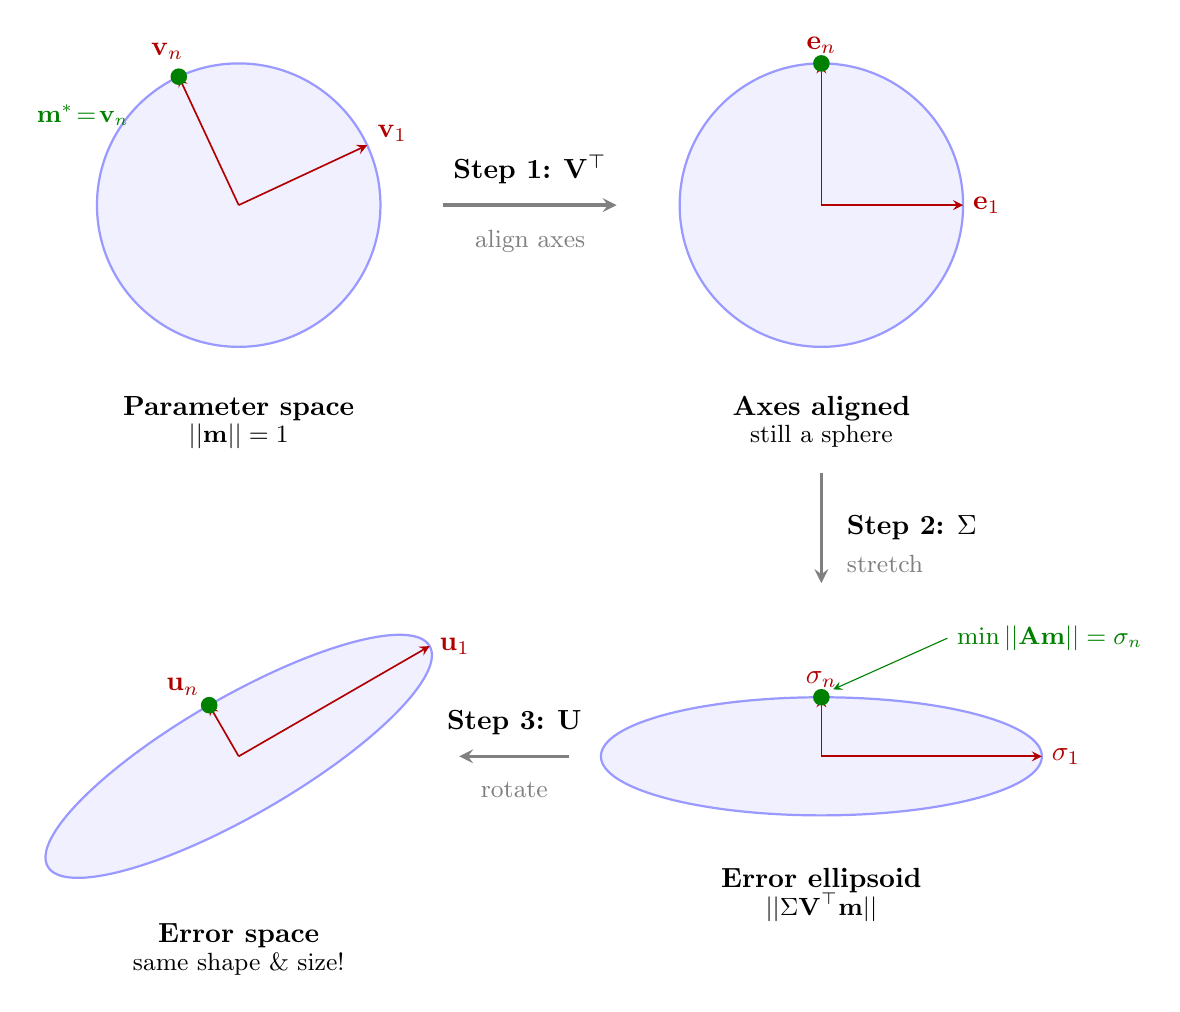
\begin{tikzpicture}[>=stealth, font=\normalsize]

  % ======== TOP ROW ========

  % === Panel 1: Unit sphere in parameter space ===
  \begin{scope}[shift={(0,3.5)}]
    \fill[blue!6] (0,0) circle (1.8);
    \draw[thick, blue!40] (0,0) circle (1.8);
    % V-basis vectors (tilted to show non-axis-aligned)
    \draw[->, semithick, red!70!black] (0,0) -- ({1.8*cos(25)},{1.8*sin(25)});
    \node[red!70!black] at ({2.15*cos(25)},{2.15*sin(25)}) {$\mathbf{v}_1$};
    \draw[->, semithick, red!70!black] (0,0) -- ({1.8*cos(115)},{1.8*sin(115)});
    \node[red!70!black] at ({2.15*cos(115)},{2.15*sin(115)}) {$\mathbf{v}_n$};
    % Green dot: optimal m at v_n
    \fill[green!50!black] ({1.8*cos(115)},{1.8*sin(115)}) circle (3pt);
    \node[green!50!black, left, font=\small] at ({1.5*cos(148)},{1.5*sin(148)+0.35}) {$\mathbf{m}^*\!=\!\mathbf{v}_n$};
    % Subtitle
    \node[below, font=\normalsize\bfseries, align=center] at (0,-2.3) {Parameter space\\[-2pt]{\normalfont\small $||\mathbf{m}||=1$}};
  \end{scope}

  % === Arrow: V^T (horizontal, top row) ===
  \draw[->, very thick, black!50] (2.6, 3.5) -- (4.8, 3.5);
  \node[above] at (3.7, 3.65) {\textbf{Step 1:} $\mathbf{V}^\top$};
  \node[below, font=\small, gray] at (3.7, 3.3) {align axes};

  % === Panel 2: Aligned unit sphere ===
  \begin{scope}[shift={(7.4,3.5)}]
    \fill[blue!6] (0,0) circle (1.8);
    \draw[thick, blue!40] (0,0) circle (1.8);
    \draw[->, semithick, red!70!black] (0,0) -- (1.8,0) node[right] {$\mathbf{e}_1$};
    \draw[->, semithick, red!70!black] (0,0) -- (0,1.8) node[above] {$\mathbf{e}_n$};
    \fill[green!50!black] (0,1.8) circle (3pt);
    \node[below, font=\normalsize\bfseries, align=center] at (0,-2.3) {Axes aligned\\[-2pt]{\normalfont\small still a sphere}};
  \end{scope}

  % === Arrow: Sigma (vertical, right side) ===
  \draw[->, very thick, black!50] (7.4, 0.1) -- (7.4, -1.3);
  \node[right, align=left] at (7.6, -0.6) {\textbf{Step 2:} $\boldsymbol{\Sigma}$};
  \node[right, font=\small, gray] at (7.6, -1.05) {stretch};

  % ======== BOTTOM ROW (right-to-left for clockwise flow) ========

  % === Panel 3: Error ellipsoid (bottom-right, under Panel 2) ===
  \begin{scope}[shift={(7.4,-3.5)}]
    \fill[blue!6] (0,0) ellipse (2.8 and 0.75);
    \draw[thick, blue!40] (0,0) ellipse (2.8 and 0.75);
    \draw[->, semithick, red!70!black] (0,0) -- (2.8,0) node[right] {$\sigma_1$};
    \draw[->, semithick, red!70!black] (0,0) -- (0,0.75) node[above] {$\sigma_n$};
    \fill[green!50!black] (0,0.75) circle (3pt);
    % Annotation arrow
    \draw[->, thin, green!50!black] (1.6, 1.5) -- (0.15, 0.85);
    \node[green!50!black, right, font=\small] at (1.6, 1.5) {$\min ||\mathbf{A}\mathbf{m}|| = \sigma_n$};
    \node[below, font=\normalsize\bfseries, align=center] at (0,-1.3) {Error ellipsoid\\[-2pt]{\normalfont\small $||\boldsymbol{\Sigma}\mathbf{V}^\top\mathbf{m}||$}};
  \end{scope}

  % === Arrow: U (horizontal, bottom row, right-to-left) ===
  \draw[->, very thick, black!50] (4.2, -3.5) -- (2.8, -3.5);
  \node[above] at (3.5, -3.35) {\textbf{Step 3:} $\mathbf{U}$};
  \node[below, font=\small, gray] at (3.5, -3.7) {rotate};

  % === Panel 4: Rotated ellipsoid in error space (bottom-left) ===
  \begin{scope}[shift={(0,-3.5)}]
    \fill[blue!6, rotate=30] (0,0) ellipse (2.8 and 0.75);
    \draw[thick, blue!40, rotate=30] (0,0) ellipse (2.8 and 0.75);
    \draw[->, semithick, red!70!black] (0,0) -- ({2.8*cos(30)},{2.8*sin(30)}) node[right] {$\mathbf{u}_1$};
    \draw[->, semithick, red!70!black] (0,0) -- ({0.75*cos(120)},{0.75*sin(120)}) node[above left] {$\mathbf{u}_n$};
    \fill[green!50!black] ({0.75*cos(120)},{0.75*sin(120)}) circle (3pt);
    \node[below, font=\normalsize\bfseries, align=center] at (0,-2.0) {Error space\\[-2pt]{\normalfont\small same shape \& size!}};
  \end{scope}

\end{tikzpicture}%
}
\end{center}

\pagebreak

\begin{subquestion}[points=3,drawbox=false]
To calibrate \textbf{Camera A}, we run \texttt{U, S, VT = np.linalg.svd(A)} on our $2N \times 12$ matrix $\mathbf{A}$ built from a photo of a 3D calibration stage with 20 point correspondences. The twelve singular values returned are:
\[
S = [\;142.5,\; 89.3,\; 71.0,\; 54.2,\; 41.8,\; 33.1,\; 19.7,\; 12.4,\; 5.6,\; 2.1,\; 0.83,\; 0.0003\;]
\]

\begin{orangebox}
Which SVD outputs give us our desired calibrated camera matrix $\mathbf{M}$? \\
Place \filled~next to all correct answers.
\end{orangebox}
\end{subquestion}

\begin{answer}[height=17]
\begin{enumerate}[(a),leftmargin=12pt]
\item \cbox~Any row of $\mathbf{V^\top}$. All are unit vectors ($||\mathbf{m}||=1$) that align the unit sphere with the principal axes, so all satisfy the scale constraint and give valid cameras.
\item \cbox~First row of $\mathbf{V^\top}$. It aligns the unit sphere with the principal axes, and corresponds to $\sigma_{1} = 142.5$.
\item \cbox~Last row of $\mathbf{V^\top}$. It aligns the unit sphere with the principal axes, and corresponds to $\sigma_{12} = 0.0003$.
\item \cbox~The diagonal vector from $S$. The singular values are the camera parameters as they encode how it stretches the scene along each axis.
\item \cbox~Any column of $\mathbf{U}$. All are unit vectors ($||\mathbf{m}||=1$) that align the ellipsoid with the error space, so all satisfy the scale constraint and give valid cameras.
\item \cbox~First column of $\mathbf{U}$. It aligns the ellipsoid with the error space, and corresponds to $\sigma_{1} = 142.5$.
\item \cbox~Last column of $\mathbf{U}$. It aligns the ellipsoid with the error space, and corresponds to $\sigma_{12} = 0.0003$.
\end{enumerate}
\end{answer}

\pagebreak

\begin{subquestion}[points=3,drawbox=false]
\noindent
\begin{minipage}[m]{0.7\linewidth}
You calibrate a second camera (\textbf{Camera B}) using a photo of a 2D calibration checkerboard with 20 corners. Here are its singular values:
\begin{gather*}
[\;310.4,\; 198.7,\; 155.2,\; 88.6,\; 61.3,\; 42.0,\; 27.5,\; \dots \\
14.1,\; 0.0006,\; 0.0004,\; 0.0002,\; 0.0001\;]
\end{gather*}
\end{minipage}%
\hfill
\begin{minipage}[m]{0.3\linewidth}
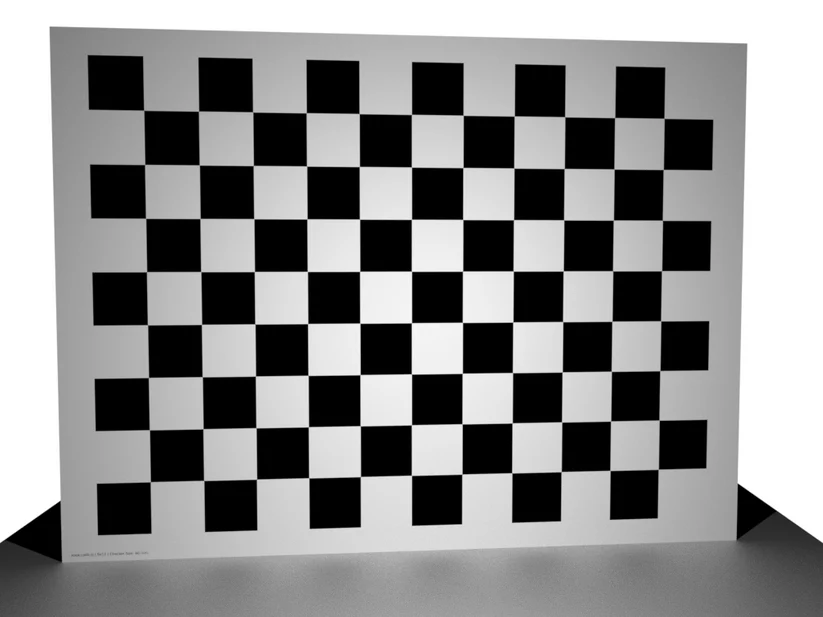
\includegraphics[width=\linewidth]{images/calibio_target.png}
\end{minipage}

Both cameras A and B have tiny algebraic residuals $||\mathbf{A}\mathbf{m}||$, yet when tested on new scene points, the reprojection error in Camera B is 200\,px.

\begin{orangebox}
\textbf{(i)} Something is wrong with Camera B's calibration. What is it, why does it cause the large reprojection error on the test point, and how can you tell from the singular values? \textbf{[3--5 sentences]}
\end{orangebox}
\end{subquestion}

\begin{answer}[height=10]
TODO: Your answer here.
\end{answer}

\begin{subquestion}[points=3]
A classmate suggests applying \emph{Hartley normalization} to reduce the reprojection error in Camera B. Place \filled~next to all correct answers.
\end{subquestion}

\begin{answer}[height=11]
\begin{enumerate}[(a), leftmargin=12pt]
\item \cbox~It will help. The issue is caused by the large magnitude mismatch between pixel coordinates and world coordinates in $\mathbf{A}$. Normalization will rescale the entries so that the SVD can resolve all 12 singular directions accurately.
\item \cbox~It will help, but only if you also add more point correspondences from the same checkerboard to overdetermine the system further.
\item \cbox~It won't help. Camera B's problem is a geometric degeneracy and no preprocessing on $\mathbf{A}$ can fix it.
\item \cbox~It won't help. Hartley normalization only applies to the 8-point algorithm for the fundamental matrix, not to the DLT for camera calibration.
\end{enumerate}
\end{answer}

\pagebreak

\textbf{SVD Summary.} Camera geometry estimation problems via DLT use the SVD everywhere: camera matrices, essential and fundamental matrices, point triangulation. Why:
\begin{itemize}[leftmargin=12pt]
    \item \textbf{Enforces the scale constraint:} It lets us search only valid solutions on the unit sphere ($||\mathbf{m}||=1$) to homogeneous problems, preventing the useless trivial solution $\mathbf{m}=0$.
    \item \textbf{Finds the optimal parameters:} The columns of $\mathbf{V}$ provide an orthogonal basis of candidate solutions for our camera matrix with known error residuals to pick from.
    \item \textbf{Quantifies the error:} The singular values ($\sigma_i$) tell us exactly what the algebraic error $||\mathbf{A}\mathbf{m}||$ will be if we choose the corresponding column of $\mathbf{V}$.
    \item \textbf{Ensures numerical stability in a computer:} It operates on $\mathbf{A}$ directly, so avoids floating-point precision loss from computing the eigenvectors of $\mathbf{A}^\top\mathbf{A}$ directly.
    \item \textbf{Handles overdetermined, non-square systems:} Our matrix $\mathbf{A}$ is typically tall and skinny as we have many point correspondences and few parameters. To solve the homogeneous form $\mathbf{A}\mathbf{m} = \mathbf{0}$, the SVD provides the approximate right null space (the last column of $\mathbf{V}$). If we instead formulate it as an inhomogeneous system $\mathbf{A}\mathbf{x} = \mathbf{b}$ (e.g., by setting $M_{3,4} = 1$), the SVD constructs the Moore-Penrose pseudoinverse $\mathbf{A}^+ = \mathbf{V}\boldsymbol{\Sigma}^+\mathbf{U}^\top$ to find the least-squares solution $\mathbf{x} = \mathbf{A}^+\mathbf{b}$. This is exactly what \texttt{lstsq} computes under the hood!
\end{itemize}

\vspace{1cm}
\textbf{Minor Python note:} \texttt{np.linalg.svd} returns a matrix called \texttt{Vh}; short for $\mathbf{V}^H$. This is the \emph{conjugate transpose} (or \emph{Hermitian}) of $\mathbf{V}$. For real-valued matrices like ours, $\mathbf{V}^H = \mathbf{V}^\top$.

%%%%%%%%%%%%%%%%%%%%%%%%%%%%%%%%%%%%%%%%%%%%%%%%%%%%%%%%%%%%%%%%%%%%%%%%
\pagebreak

\begin{question}[points=14,drawbox=false]
In the code, you will consider depth from two camera views using two pipelines that rely on \emph{homographies} in different ways:

\begin{itemize}[leftmargin=12pt]
    \item \textbf{Part A (Calibrated):} Given projection matrices $\mathbf{M}$, the \emph{plane-sweep} algorithm warps Camera 1's image into Camera 2's view via a depth-dependent homography $\mathbf{H}(\lambda)$ to help us match.
    \item \textbf{Part B (Uncalibrated):} Given only feature point correspondences, we can estimate the fundamental matrix $\mathbf{F}$ and from that derive \emph{rectifying homographies} $\mathbf{H}_1, \mathbf{H}_2$ to help us match.
\end{itemize}
Both pipelines recover scene geometry information but with different guarantees. What can each approach tell us about the scene?

This is challenging! \emph{Draw these out visually} and use the \emph{livePlaneSweep.py} demo to help your understanding.
\end{question}

\begin{subquestion}[points=2]
\textbf{Warm-up:} Which scenarios cause \emph{both} the calibrated and the uncalibrated pipelines to fail to estimate scene geometry? \\
Place \filled~next to all correct answers.
\end{subquestion}

\begin{answer}[height=13]
    \begin{enumerate}[(a),leftmargin=12pt]
    \item \cbox~Scenes where all objects are more than 100\,m away. Both methods require nearby geometry.
    \item \cbox~Scenes with textureless regions. Both methods rely on local photometric matching to establish correspondences, and a uniform surface provides no distinctive pattern.
    \item \cbox~Scenes lit by a single point light source. Both methods require complex multi-directional illumination.
    \item \cbox~Cameras with different focal lengths. Both methods require identical intrinsics (even if they are unknown).
    \item \cbox~Cameras placed at the same position with different orientations. With zero baseline there is no parallax, so neither method can recover depth.
\end{enumerate}
\end{answer}

\pagebreak

\paragraph{Part A: Calibrated.}
In lecture, we saw that we can write each camera as $\mathbf{M} = [\mathbf{A} \;|\; \mathbf{t}]$ with camera center $\mathbf{C} = -\mathbf{A}^{-1}\mathbf{t}$. A pixel in Camera 1 $\mathbf{p} = [u, v, 1]^\top$ back-projects to the 3D point $\mathbf{P} = \mathbf{C}_\text{1} + \lambda\, \mathbf{A}_\text{1}^{-1}\mathbf{p}$ along ray $\mathbf{r}=\mathbf{A}_\text{1}^{-1}\mathbf{p}$, with $\mathbf{p}$ at depth $\lambda$. Projecting $\mathbf{P}$ into Camera 2 gives a depth-dependent homography:
%
\begin{equation*}
\mathbf{H}(\lambda) = \lambda\, \mathbf{B} + \mathbf{a}\, \mathbf{e}_3^\top, \qquad \mathbf{B} = \mathbf{A}_\text{2}\, \mathbf{A}_\text{1}^{-1}, \qquad \mathbf{a} = \mathbf{A}_\text{2}\, \mathbf{C}_\text{1} + \mathbf{t}_\text{2}
\end{equation*}
%
This geometric relationship is used by the fronto-parallel \emph{plane-sweep algorithm} to evaluate $\mathbf{H}(\lambda)$ at many candidate depths. We warp Camera 1's \emph{screen space point coordinates} into Camera 2's view. Then, in \emph{pixel intensity space}, we measure local patch agreement by some metric like normalized cross-correlation (NCC). For each point, the best depth $\lambda$ is kept.

\begin{subquestion}[points=2]
$\mathbf{H}(\lambda)$ is a single $3\times3$ matrix applied to Camera 1's coordinates. For which screen space points does this geometric warping produce the correct correspondence in Camera 2? \\
Place \filled~next to all correct answers.
\end{subquestion}

\begin{answer}[height=11]
\begin{enumerate}[(a),leftmargin=12pt]
\item \cbox~All points, because $\mathbf{H}(\lambda)$ is derived from the full projection matrices of both cameras and so every point has correct depth.
\item \cbox~Points near the image center, where the pinhole model is most accurate.
\item \cbox~Points whose depth is close to $\lambda$. The homography is a local approximation that holds for points near that depth and degrades for farther points.
\item \cbox~Points whose depth is $\lambda$. The homography is geometrically exact only for points at that depth.
\item \cbox~Points with sufficient local texture in the pixel image, because $\mathbf{H}(\lambda)$ needs texture gradients to determine where each pixel maps.
\end{enumerate}
\end{answer}

\pagebreak

\begin{subquestion}[points=4]
As the depth plane approaches Camera 1's center ($\lambda \to 0$), $\mathbf{H}(\lambda) \to \mathbf{a}\,\mathbf{e}_3^\top$. This means that every Camera 1 point $\mathbf{p}$ converges to the same location $\mathbf{a}$ in Camera 2.
Where is $\mathbf{a}$ geometrically? \\
Place \filled~next to all correct answers.
\end{subquestion}

\begin{answer}[height=10]
\begin{enumerate}[(a),leftmargin=12pt]
\item \cbox~All points converge to the \textbf{principal point} of the other camera, because at zero depth the image becomes infinitely small.
\item \cbox~All points converge to the \textbf{midpoint} between the two camera centers, since at zero depth the scene is ``between'' the cameras.
\item \cbox~All points converge to the \textbf{epipole} of Camera 1 in Camera 2, because at zero depth every back-projected ray collapses to Camera 1's center $\mathbf{C}_\text{1}$.
\item \cbox~All points converge to an \textbf{undefined} location because $\mathbf{H}(\lambda)$ is singular ($\det = 0$), so the limit has no geometric meaning.
\end{enumerate}
\end{answer}


%%%%%%%%%%%%%%%%%%%%%%%%%%%%%%%%%%%%%%%%%%%%%%%%%%%%%%%%%%%%%%%%%%%%%%%%
\pagebreak

\paragraph{Part B: Uncalibrated.}
Without known camera matrices $\mathbf{M}$, we estimate the $3 \times 3$ fundamental matrix $\mathbf{F}$ from 2D--2D point correspondences. It satisfies the \emph{epipolar constraint}: for corresponding points $\mathbf{x}$ and $\mathbf{x}'$,
%
\begin{equation*}
{\mathbf{x}'}^\top \mathbf{F}\, \mathbf{x} = 0
\end{equation*}
%
The product $\mathbf{l}' = \mathbf{F}\, \mathbf{x}$ is the \emph{epipolar line} in image~2 on which the correspondence $\mathbf{x}'$ must lie.

\begin{subquestion}[points=2]
From $\mathbf{F}$, we can compute \emph{rectifying homographies} $\mathbf{H}_1$ and $\mathbf{H}_2$ that help with dense matching.
What do these homographies accomplish? \\
Place \filled~next to all correct answers.
\end{subquestion}

\begin{answer}[height=11]
\begin{enumerate}[(a),leftmargin=12pt]
    \item \cbox~They warp both images so that each point's correspondence appears at the same image coordinates, eliminating the need for further matching.
    \item \cbox~They decompose $\mathbf{F}$ into the cameras' relative rotation and translation, so that correspondences can be triangulated directly.
    \item \cbox~They warp both images to remove radial lens distortion, since $\mathbf{F}$ was estimated from distorted measurements, so that we can match along 1D epipolar lines.
    \item \cbox~They warp both images so that each point's correspondence lies on the same horizontal row, so that we can match along 1D epipolar lines.
\end{enumerate}
\end{answer}


\begin{subquestion}[points=4]
After rectification, the disparity $d$ at a pixel is the offset to its correspondence. For calibrated cameras with baseline $b$ and focal length $f$, depth satisfies $Z = bf/d$. In Part~B (uncalibrated), you estimate $\mathbf{F}$ from 2D correspondences alone and then rectify. Which statements about the recovered disparity are correct? \\
Place \filled~next to all correct answers.
\end{subquestion}

\begin{answer}[height=11]
\begin{enumerate}[(a),leftmargin=12pt]
    \item \cbox~Disparity is proportional to depth: closer objects have smaller disparity.
    \item \cbox~Disparity is inversely proportional to depth: closer objects have larger disparity.
    \item \cbox~Disparity from uncalibrated rectified images has no systematic relationship to depth, because the rectifying homographies introduce arbitrary distortion.
    \item \cbox~Disparity after rectification can give metric depth, because the rectifying homographies standardize the geometry.
    \item \cbox~Disparity after rectification can give relative depth, because $b$ and $f$ are unknown.
\end{enumerate}
\end{answer}


%%%%%%%%%%%%%%%%%%%%%%%%%%%%%%%%%%%
\pagebreak

\writefeedback

\end{document}
